\documentclass{article}
\usepackage{float}
\usepackage[polish]{babel}
\usepackage[utf8]{inputenc}
\usepackage{polski}
\usepackage{listings} %code environment
\frenchspacing
\setcounter{tocdepth}{2}
\usepackage{graphicx}
\graphicspath{ {images/} }
\usepackage{color}

\lstdefinestyle{main}{
	keywords={
		after, always, causes, if, impossible, initially, observable, 
		partakes, releases, typically
    },
    keywordstyle={\bfseries},
    keywordstyle=[2]\textsc,
    frame=single,
}

\begin{document}
	
\begin{titlepage}

\newcommand{\HRule}{\rule{\linewidth}{0.5mm}}
\newcommand{\Action}[1]{\textsc{#1}}

\center

%----------------------------------------------------------------------------------------

\textsc{\LARGE Politechnika Warszawska}\\[0.3cm]
\textsc{\Large Wydział Matematyki i Nauk Informacyjnych}\\[0.6cm]

% logo

\includegraphics[width=2cm, height=2cm]{logo}\\[0.6cm]


\textsc{\Huge Reprezentacja wiedzy}\\[0.3cm]

%----------------------------------------------------------------------------------------

\HRule \\[0.4cm]
{ \LARGE \bfseries Raport z testów projektu grupy nr 1}\\[0.1cm]
 
%----------------------------------------------------------------------------------------

\HRule \\[0.4cm]
{  \bfseries Programy działań z efektami domyślnymi}\\[1.2cm]

% authors
\begin{flushright}
\Large \emph{Autorzy:}\\[0.5cm]
Dragan Łukasz\\
Flis Mateusz\\
Izert Piotr\\
Pielat Mateusz\\
Rząd Przemysław\\
Siry Roman\\
\textbf{Waszkiewicz Piotr}\\
Zawadzka Anna\\[0.9cm]

\end{flushright}

% date
\vfill
{\large 14 czerwca 2016}\\[1cm]
	


\end{titlepage}
	
\newpage

\section{Opis projektu}
Tematem testowanego przez nas projektu są programy działań z efektami domyślnymi. Rozpatrywana klasa systemów dynamicznych spełnia następujące warunki:
\begin{itemize}
	\item Prawo inercji
	\item Niedeterminizm i sekwencyjność działań
	\item Pełna informacja o wszystkich akcjach i wszystkich ich skutkach bezpośrednich
	\item Z każdą akcją związany jest:
	\begin{enumerate}
		\item Warunek początkowy (ew. true)
		\item Efekt akcji
		\item Jej wykonawca
	\end{enumerate}
	\item Skutki akcji:
	\begin{enumerate}
		\item Pewne (zawsze występują po zakończeniu akcji)
		\item Domyślne (preferowane. Zachodzą po zakończeniu akcji, o ile nie jest wiadomym, że nie występują)
	\end{enumerate}
	\item Efekty akcji zależą od jej stanu, w którym akcja się zaczyna i wykonawcy tej akcji
	\item W pewnych stanach akcje mogą być niewykonalne przez pewnych (wszystkich) wykonawców
\end{itemize}

Opracowywany jezyk kwerend ma za zadanie umożliwiać tworzenie zapytań,
pozwalających na uzyskanie odpowiedzi na następujace pytania:
\begin{itemize}
	\item Czy podany program działań jest wykonywalny zawsze/kiedykolwiek?
	\item Czy wykonanie podanego programu działań z dowolnego stanu spełniającego warunek $\pi$ prowadzi zawsze/kiedykolwiek/na ogół do stanu spełniającego warunek celu $\gamma$ ?
	\item Czy z dowolnego stanu spełniającego warunek $\pi$ cel $\gamma$ jest osiągalny zawsze/kiedykolwiek/na ogół?
	\item Czy wskazany wykonawca jest zaangażowany w realizację programu zawsze/kiedykolwiek?
\end{itemize}
\newpage

\section{Przeprowadzone testy}
\subsection{Test 1}
Zdefiniowana dziedzina:
\bigskip
\lstset{
	style=main,
	keywords=[2]{Load, Shoot},
}
\begin{lstlisting}[mathescape=true]
initially $\neg$ painted
(PAINT, (MALARZ)) causes painted
(CLEAR, (MALARZ, INFORMATYK)) causes $\neg$ painted
\end{lstlisting}
\vspace{1cm}
Otrzymany w wyniku zbudowania dziedziny graf wyglądał następująco:

\begin{figure}[H]
\centering
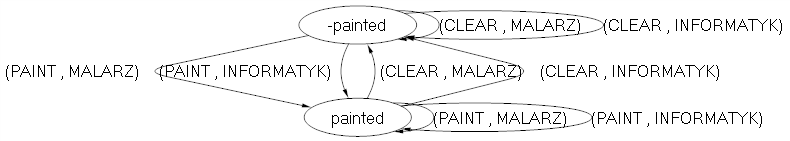
\includegraphics[scale=0.6]{test1_graf}
\end{figure}

Jak widać zdefiniowane w nim zostały przejścia dla akcji PAINT wykonanej przez aktora INFORMATYK, prowadzące ze stanu w którym obraz nie był namalowany ($\neg$ painted) do stanu w którym już istniał (painted). Jest to błąd w programie.

\newpage

\end{document}
